\documentclass[a4paper,11pt]{article}
\usepackage[francais]{babel}
\usepackage[utf8]{inputenc}
\usepackage[T1]{fontenc}
\usepackage{graphicx}
\usepackage{geometry}
\usepackage{amsmath}
\usepackage{float}
\usepackage{listings}
\usepackage{xcolor}
\usepackage{hyperref}

\setcounter{secnumdepth}{0}
\hypersetup{colorlinks=true, linkcolor=black}
\geometry{margin=1in}

\begin{document}

\selectlanguage{french}

\begin{titlepage}
    \begin{center}
        % Logo de l'école en en-tête
        
\includegraphics[width=5cm]{./img/uqac.png}\\[1cm]
        
        % Titre principal
        \vspace*{1cm} % Ajuster pour centrer verticalement
        {\Huge \textbf{Interaction Humain-Robot : Devoir 2}\\[0.5cm]}

        % Image de couverture (centrée en dessous du logo)
        \vspace*{1cm}
        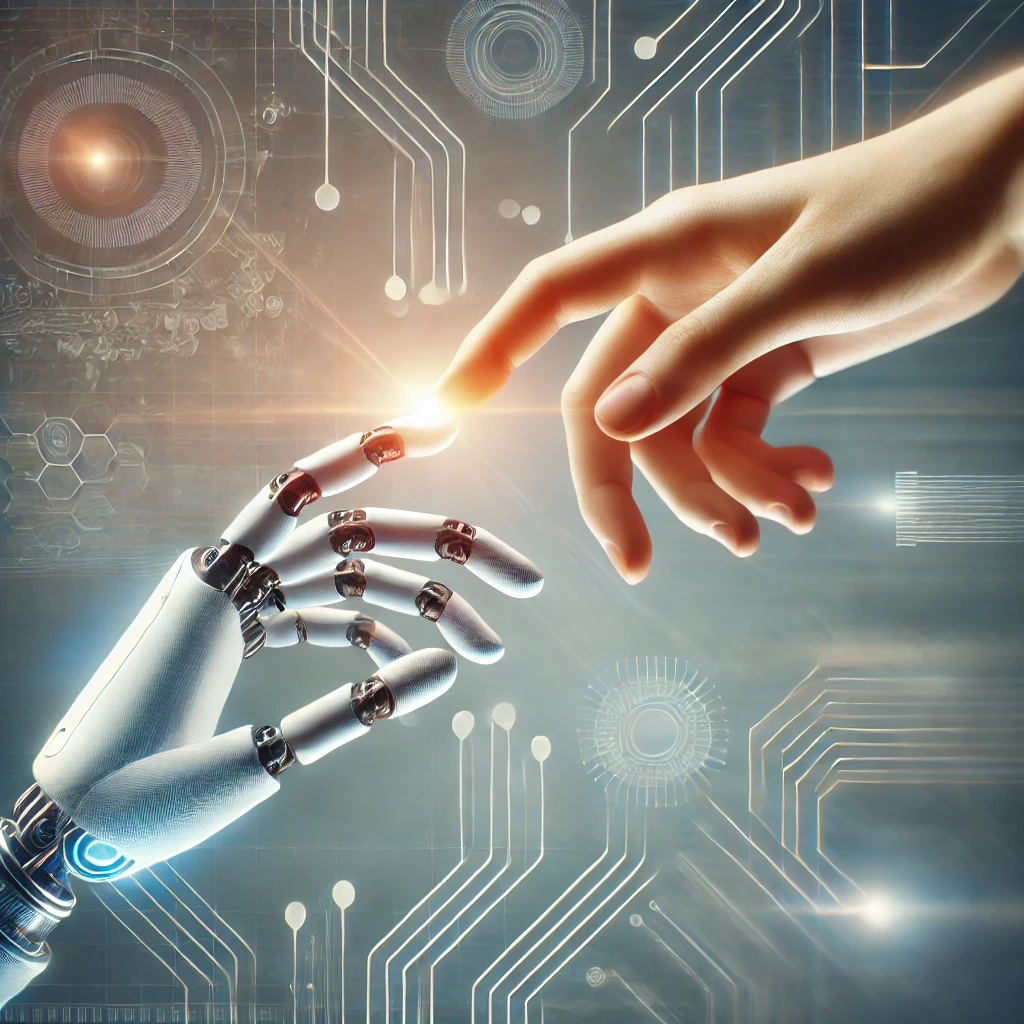
\includegraphics[width=0.7\textwidth]{./img/image_IHR.png}\\[1cm]

        
        
        % Informations des auteurs
        \vspace{2cm}
        {\LARGE Constance ALOYAU, Erwan MAWART, Benjamin PELLIEUX}
        
        \vspace{0.5cm}
        {\large PELB28120100, MAWE14050200, ALOC25530200}
        
        % Date
        \vspace{2cm}
        {\Large \today}
        
        \vfill
    \end{center}
\end{titlepage}

\tableofcontents
\newpage

\section*{Introduction}
    Les vibrations dans un mécanisme robotique, lorsqu’il est manipulé par un opérateur humain, peuvent affecter significativement la qualité et la précision de la tâche réalisée. Nous étudions l'impact perceptuel de ces vibrations lorsqu’un opérateur applique une force à l’aide d’une poignée sur un capteur de force fixé à un robot à un degré de liberté...

\section{Énoncé 1 : Conception du modèle du mécanisme}
\subsection{    Question 1.1 : Modèle variable d’états pour l’IAD}
% Inclure les figures et les résultats de l'analyse de la bande passante
\begin{figure}[h!]
    \centering
    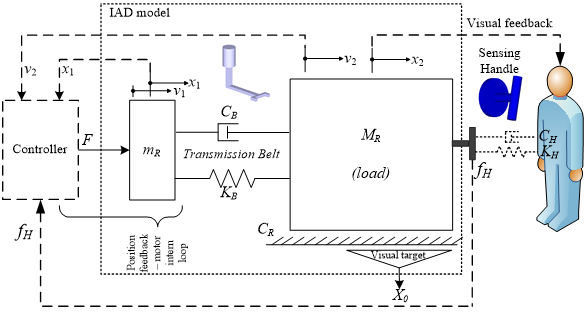
\includegraphics{./img/modele_humain-meca_robotique.png}
    \caption{Modèle du mécanisme robotique et de l'humain\label{fig:modele_humain-meca_robotique}}
\end{figure}

On note sur la \autoref{fig:modele_humain-meca_robotique} que les variables d'états sont x_{1}\end, x_{2}\end, v_{1}\end et v_{2}\end. En effet, une vitesse est la dérivée d'une position, d'où :
\begin{center}
    \begin{pmatrix}
        x_{1}\\
        x_{2}\\
        v_{1}\\
        v_{2}
    \end{pmatrix}
    =
    \begin{pmatrix}
        x_{1}\\
        x_{2}\\
        \dot{x_{1}}\\
        \dot{x_{2}}
    \end{pmatrix}
\end{center}

Ainsi, on déduit les deux équations suivantes.
\begin{center}
    \left\{\begin{matrix}
        m_{R}\ddot{x_{1}}=F-K_{B}x_{1}+K_{B}x_{2}-C_{B}\dot{x_{1}}+C_{B}\dot{x_{2}}\\
        M_{R}\ddot{x_{2}}=K_{B}x_{1}-K_{B}x_{2}+C_{B}\dot{x_{1}}-C_{B}\dot{x_{2}}-C_{R}\dot{x_{2}}\\
    \end{matrix}\right.\\
    \Leftrightarrow
    \left\{\begin{matrix}
        \ddot{x_{1}}=\frac{F-K_{B}x_{1}+K_{B}x_{2}-C_{B}\dot{x_{1}}+C_{B}\dot{x_{2}}}{m_{R}}\\
        \ddot{x_{2}}=\frac{K_{B}x_{1}-K_{B}x_{2}+C_{B}\dot{x_{1}}-C_{B}\dot{x_{2}}-C_{R}\dot{x_{2}}}{M_{R}}
    \end{matrix}\right.\\
\end{center}

Les variables d'état se constitue de deux équations matricielles : $\dot{X}=AX+BU$ et $Y=CX+DU$, où $A$, $B$, $C$ et $D$ sont à déterminées.
\begin{center}
    $\dot{X}=AX+BU$
    \Leftrightarrow
    \begin{bmatrix}
        \dot{x_{1}}\\
        \dot{x_{2}}\\
        \ddot{x_{1}}\\
        \ddot{x_{2}}
    \end{bmatrix}
    =
    \begin{bmatrix}
        0 & 0 & 1 & 0\\
        0 & 0 & 0 & 1\\
        \frac{-K_{B}}{m_{R}} & \frac{K_{B}}{m_{R}} & \frac{-C_{B}}{m_{R}} & \frac{C_{B}}{m_{R}}\\
        \frac{K_{B}}{M_{R}} & \frac{-K_{B}}{M_{R}} & \frac{C_{B}}{M_{R}} & \frac{-(C_{B}+C_{R})}{M_{R}}\\
    \end{bmatrix}
    \begin{bmatrix}
        x_{1}\\
        x_{2}\\
        \dot{x_{1}}\\
        \dot{x_{2}}
    \end{bmatrix}
    +
    \begin{bmatrix}
        0 & 0 & 0 & 0\\
        0 & 0 & 0 & 0\\
        0 & 0 & \frac{1}{m_{R}} & 0\\
        0 & 0 & 0 & 0\\
    \end{bmatrix}
    \begin{bmatrix}
        0\\
        0\\
        F\\
        0
    \end{bmatrix}\\
\end{center}

\begin{center}
    $Y=CX+DU$
    \Leftrightarrow
    $Y=CX$
    \Leftrightarrow
    \begin{bmatrix}
        0\\
        x_{2}\\
        0\\
        \dot{x_{2}}
    \end{bmatrix}
    =
    \begin{bmatrix}
        0 & 0 & 0 & 0\\
        0 & 1 & 0 & 0\\
        0 & 0 & 0 & 0\\
        0 & 0 & 0 & 1\\
    \end{bmatrix}
    \begin{bmatrix}
        x_{1}\\
        x_{2}\\
        \dot{x_{1}}\\
        \dot{x_{2}}
    \end{bmatrix}\\
\end{center}

\subsection{    Question 1.2 : Filtrage fréquentiel}
% Décrire les filtres appliqués, leurs ordres et l'impact sur le signal

\subsection{    Question 1.3 : Observation et la méthode d’adaptation}
% Décrire les filtres appliqués, leurs ordres et l'impact sur le signal

\section{Énoncé 2 : Simulation}
\subsection{    Question 2.1 : Utilisation de la STFT}
% Expliquer l'application de la STFT pour identifier les fréquences de vibration

\subsection{    Question 2.2 : Justification de l’utilisation des filtres}
% Justifier l'utilisation des filtres et présenter les choix effectués

\subsection{    Question 2.3 : Calcul de l'indice de vibration}
% Proposer et expliquer le calcul de l'indice de vibration en fonction des fréquences identifiées

\section{Annexe}
\subsection{Lien vers le Dépôt GitHub}
\url{https://github.com/BlueWan14/Cours_IHR/tree/main/Devoir_2}

\end{document}
